\documentclass[12pt]{article}
\usepackage[hungarian]{babel}
\selectlanguage{hungarian}
\usepackage[utf8]{inputenc}
\usepackage[T1]{fontenc}

\pdfpageheight\paperheight
\pdfpagewidth\paperwidth
\setlength\topmargin{-1cm} \setlength\oddsidemargin{-0cm}
\setlength\textheight{25cm} \setlength\textwidth{15.8cm}
\setlength\columnsep{0.25in}  \newlength\titlebox \setlength\titlebox{2.00in}
\setlength\headheight{5pt}   \setlength\headsep{0pt}
\setlength\footskip{1cm}
\setlength\leftmargin{0.0in}

\usepackage{alltt}

\usepackage{tikz}
\usetikzlibrary{shapes,shapes.geometric,shapes.multipart,calc,positioning}
\usepackage{amsmath}
\usepackage{subfig}
\date{}
\title{7. gyakorlat -- Amortizált költségelemzés és Fibonacci kupacok}
\begin{document}

\maketitle 

\noindent 1. Műveletek $n$ hosszú sorozatát végezzük el egy 
adatszerkezeten. Az $i$-edik művelet költsége $i$, ha $i$ éppen
kettőhatvány, máskülönben $1$. Mennyi az adatszerkezet műveletenkénti 
amortizációs költsége?

$$ c_i=\begin{cases}
i,& \text{ha i kettőhatvány}\\
1,& \text{különben.} \\
\end{cases} $$

Emlékeztetőül a mértani sorok összegképlete: $\sum\limits_{i=0}^n q^i = 
\frac{q^{n+1}-1}{q-1}$\\
$n$ műveletre: $\sum\limits_{i=1}^n c_i \leq n 
+ \sum\limits_{j=0}^{\lfloor \log{n} \rfloor}
2^j = n + 2n - 1 < 3n = O(n)$, vagyis műveletenként $O(1)$.

\vspace{1em}

\noindent 2.
Szúrjuk be egy üres Fibonacci kupacba az alábbi elemeket: 16, 32, 81, 2, 14, 
66, 15, 23, 44, 30.

\begin{figure}[!ht]
	\centering
	\begin{tikzpicture}
	[-,thick,every node/.style={shape=circle,inner sep=1pt,draw,thick,minimum 
	width=1.5em}]
	\node (a) at (0,0) {32};
	\node (b) at (1,0) {81};
	\node (c) at (2,0) {14};
	\node (d) at (3,0) {66};
	\node (e) at (4,0) {15};
	\node (f) at (5,0) {23};
	\node (g) at (6,0) {44};
	\node (h) at (7,0) {30};
	\node (i) at (8,0) {2};
	\node (j) at (9,0) {16};

	\path
	\foreach \startNode/\endNode in {a/b,b/c,c/d,d/e,e/f,f/g,g/h,h/i,i/j}{
		(\startNode) edge[-,thick] (\endNode)
	};
	\node[draw=none,above of=i] (i1){min};
	\draw [->] (i1) to(i);
	\end{tikzpicture}
\end{figure}

Hajtsunk végre két {\scshape Sorból()} műveletet!

\begin{figure}[!ht]
	\centering
	\subfloat[Első {\scshape Sorból()}]{
	\begin{tikzpicture}
	[-,thick,every node/.style={shape=circle,inner sep=1pt,draw,thick,minimum 
		width=1.5em}]
	\node (a) at (0,0) {16};
	\node (b) at (4,0) {14}
		child{node {15} child{node{30} child{ node{44}}} child{node{23}}}
		child{node {32} child{ node{81}}}
		child{node {66}};

	\path
	\foreach \startNode/\endNode in {a/b}{
		(\startNode) edge[-,thick] (\endNode)
	};
	\node[draw=none,above of=b] (b1){min};
	\draw [->] (b1) to(b);
	\end{tikzpicture}
	}\hfill
	\subfloat[Második {\scshape Sorból()}]{
	\begin{tikzpicture}
	[-,thick,every node/.style={shape=circle,inner sep=1pt,draw,thick,minimum 
		width=1.5em}]
	\node (a) at (0,0) {15} child{node{16} child{node {32} child{node{81}}} 
	child{node{66}}} 
	child{node{30} 
	child{ node{44}}} 
	child{node{23}};
	\node[draw=none,above of=a] (a1){min};
	\draw [->] (a1) to(a);
	\end{tikzpicture}
	}
	\caption{A {\scshape Sorból()} műveletek végrehajtásának eredménye.}
\end{figure}

\pagebreak
Hajtsuk végre az alábbi műveleteket: {\scshape Töröl(66)}, {\scshape  
Töröl(32)}, {\scshape Töröl(44)}

\begin{figure}[!ht]
	\centering
	\subfloat[{\scshape Töröl(66)}]{
	\begin{tikzpicture}
[-,thick,every node/.style={shape=circle,inner sep=1pt,draw,thick,minimum 
	width=1.5em}]
\node (a) at (0,0) {15} child{node[fill=black!40]{16} child{node {32} 
child{node{81}}} 
	child[missing]}
child{node{30} child{ node{44}}} 
child{node{23}};
\node[draw=none,above of=a] (a1){min};
\draw [->] (a1) to(a);
\end{tikzpicture}
	}
	\hfill
	\subfloat[{\scshape Töröl(32)}]{
	\begin{tikzpicture}
	[-,thick,every node/.style={shape=circle,inner sep=1pt,draw,thick,minimum 
		width=1.5em}]

	\node (a) at (0,0) {15}
	child[missing]
	child{node{30} child{ node{44}}}
	child{node{23}};
	\node (b) at (-2,0) {16} child{ node {81}};
	\path
	\foreach \startNode/\endNode in {b/a}{
		(\startNode) edge[-,thick] (\endNode)
	};
	
	\node[draw=none,above of=a] (a1){min};
	\draw [->] (a1) to(a);
	\end{tikzpicture}
	}
	\hfill
	\subfloat[{\scshape Töröl(44)}]{
	\begin{tikzpicture}
[-,thick,every node/.style={shape=circle,inner sep=1pt,draw,thick,minimum 
	width=1.5em}]

\node (a) at (0,0) {15}
child[missing]
child{node[fill=black!40]{30}}
child{node{23}};
\node (b) at (-2,0) {16} child{ node {81}};
\path
\foreach \startNode/\endNode in {b/a}{
	(\startNode) edge[-,thick] (\endNode)
};

\node[draw=none,above of=a] (a1){min};
\draw [->] (a1) to(a);
\end{tikzpicture}
	}
	\caption{A Fibonacci kupac törlések utáni állapota.}
\end{figure}

A törlések után kapott kupacot egyesítsük az alábbi Fibonacci kupaccal.
\begin{figure}[!ht]
	\centering
	\subfloat[$H_2$]{
	\begin{tikzpicture}
	[-,thick,every node/.style={shape=circle,inner sep=1pt,draw,thick}]
	\node (a) at (0,0) {42}
	child {node {75}};

	\node (b) at (2,0) {22};
	\node (c) at (4,0) {12};
	\path
	\foreach \startNode/\endNode in {a/b,b/c}
	{
		(\startNode) edge[-,thick] (\endNode)
	};
	\node[draw=none,above of=c](c1){min};
	\draw [->] (c1) to(c);
	\end{tikzpicture}
} \hfill
\subfloat[{\scshape Egyesít}($H_1$, $H_2$) eredménye]{
	\begin{tikzpicture}
	[-,thick,every node/.style={shape=circle,inner sep=1pt,draw,thick}]
	\node (a) at (0,0) {42}
	child {node {75}};
	
	\node (b) at (1.5,0) {22};
	\node (c) at (3,0) {12};
	\node (d) at (4.5,0) {16} child{ node {81}};
	\node (e) at (6,0) {15}
child[missing]
child{node[fill=black!40]{30}}
child{node{23}};
	\path
	\foreach \startNode/\endNode in {a/b,b/c,c/d,d/e}
	{
		(\startNode) edge[-,thick] (\endNode)
	};
	\node[draw=none,above of=c](c1){min};
	\draw [->] (c1) to(c);
	\end{tikzpicture}
}
\end{figure}

Végül hajtsunk végre egy {\scshape Sorból}() műveletet, majd módosítsuk a 42
kulcsot 11-re.

\begin{figure}[!ht]
	\centering
	\subfloat[{\scshape Sorból}() után]{
	\begin{tikzpicture}
	[-,thick,every node/.style={shape=circle,inner sep=1pt,draw,thick,minimum 
		width=1.5em}]
	\node (a) at (0,0) {22};
	\node (b) at (2,0) {15} child{node{16} child{node {42} child{node{75}}} 
		child{node{81}}} 
	child{node[fill=black!40]{30}} 
	child{node{75}};
	\node[draw=none,above of=a] (a1){min};
	\draw [->] (a1) to(a);
	\path
	\foreach \startNode/\endNode in {a/b}
	{
		(\startNode) edge[-,thick] (\endNode)
	};
	\end{tikzpicture}
	}
    \hfill
   	\subfloat[{\scshape Sorból}() után]{
   			\begin{tikzpicture}
   		[-,thick,every node/.style={shape=circle,inner 
   		sep=1pt,draw,thick,minimum 
   			width=1.5em}]
   		\node (c) at(-2,0) {11} child{node{75}};
   		\node (a) at (0,0) {22};
   		\node (b) at (2,0) {15} child{node[fill=black!40]{16} 
   		child[missing] child{node{81}}} 
   		child{node[fill=black!40]{30}} 
   		child{node{75}};
   		\node[draw=none,above of=c] (c1){min};
   		\draw [->] (c1) to(c);
   		\path
   		\foreach \startNode/\endNode in {c/a,a/b}
   		{
   			(\startNode) edge[-,thick] (\endNode)
   		};
   		\end{tikzpicture}
   	}
\end{figure}

Az utolsó {\scshape Sorból}() műveletet követően mennyi a Fibonacci kupac 
potenciálfüggvényének az értéke? $\Phi(H) = t(H) + 2m(H) = 3 + 2*2=7$

\end{document}